\section*{Test 10 Allocation of escape routes}

Construct the section of a corridor as shown in Figure 10 with a population of adults from Figure 5 with an immediate reaction and distribute the walking speeds over a population of 23 persons. The persons in rooms 1, 2, 3, 4, 7, 8, 9 and 10 are assigned to the main exit, with all other persons assignedthe secondary exit. The expected result is that all allocated persons go to their corresponding exits.



\begin{figure}[h]
	\centering
	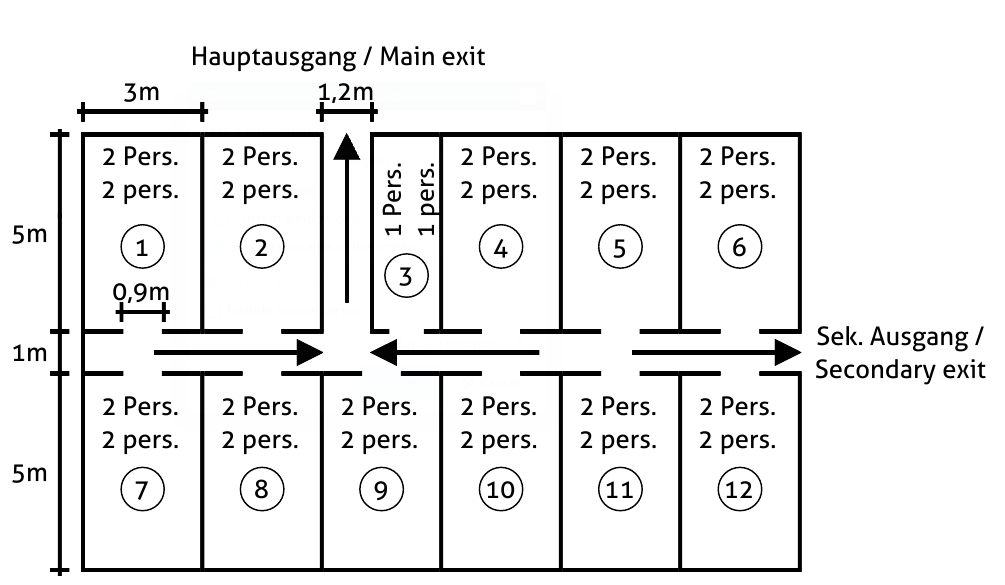
\includegraphics[scale=0.5]{test_description/Corridor_test_10.png}
	\caption{\footnotesize \textbf{Corridor with adjacent rooms}}
\end{figure}

